\documentclass{article}                                                                                   \usepackage{amsmath, amssymb}
\usepackage{geometry}
\usepackage{graphicx}
\usepackage{float}

\begin{document}

\section*\textbf{Geometry Question .}
\begin{enumerate}
\item In Figure 1, $\angle BAC = 90^\circ$. $AD$ $\parallel$ $BC$. Prove that $AB^2 + CD^2 = BD^2 + AC^2$.
        \begin{figure}[h]
        \centering
                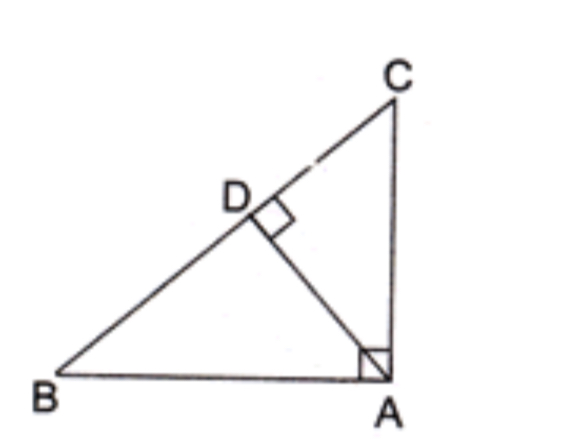
\includegraphics[width=70mm]{./images/IMG01.PNG}
                \caption{1}                                                                                               \label{fig}                   
         \end{figure}
\item  In Figure 2, $PT = 6 \text{ cm}$, $AR = 5 \text{ cm}$. Find the length of $PA$.

\begin{figure}[h]
        \centering
                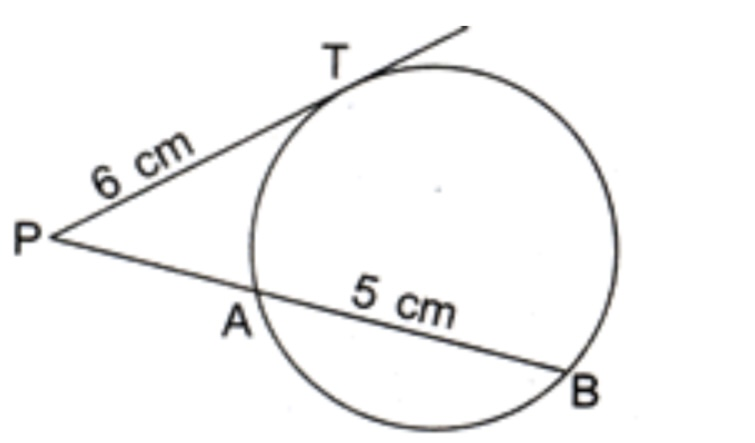
\includegraphics[width=70mm]{./images/IMG02.PNG}
                \caption{2}
                \label{fig:}
\end{figure}

                                                             \item Draw the graphs of the following equations:
$3x - 4y + 6 = 0 ,3x + y - 9 = 0$
Also, determine the co-ordinates of the vertices of the triangle formed by these lines and the x
axis.
\item  A solid is in the form of a right circular cylinder with hemispherical ends. The total height
of the solid is 58 cm and the diameter of the cylinder is 28cm. Find the total surface area of the
   solid  $\pi \approx \frac{22}{7} $

\item . Construct a triangle $ABC$ in which $BC$ = 7 cm, and median $AD$ = 5 cm, $\angle A=60^\circ$ Write      the steps of construction also.

\begin{figure}[h]                                                                                                 \centering
                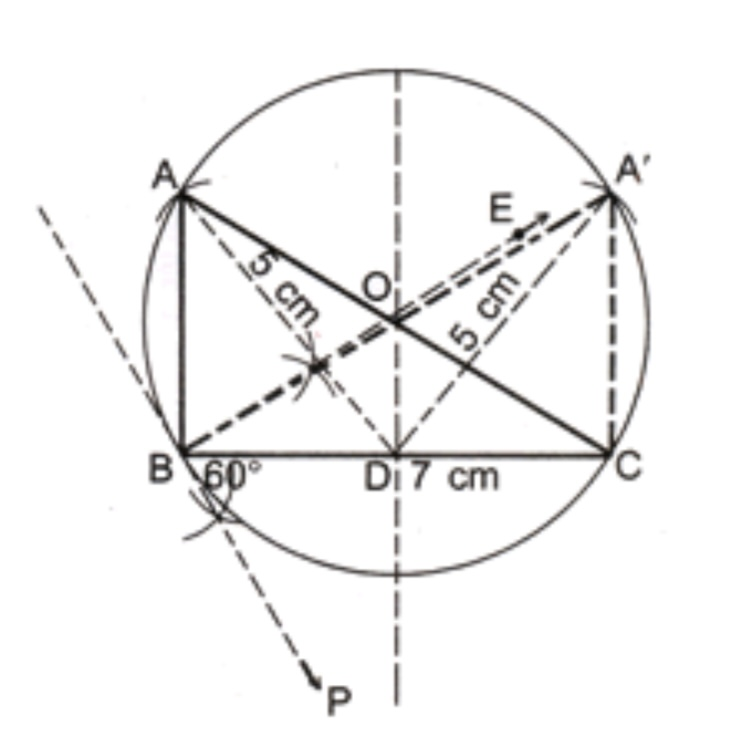
\includegraphics[width=70mm]{./images/IMG04.PNG}                                                     \caption{3}
                 \label{fig:}                                                                       \end{figure}.
\item Show that the points A(6, 2), B(2, 1), C(1, 5) and D(5, 6) are the vertices of a square

\item Find the value of p for which the points (- 5, 1), (1, p) and \(4, - 2\) are collinear.
\item . Prove that in a right triangle, the square of the hypotenuse is equal to the sum of the
squares of the other two sides.
\begin{figure}[h]
        \centering
          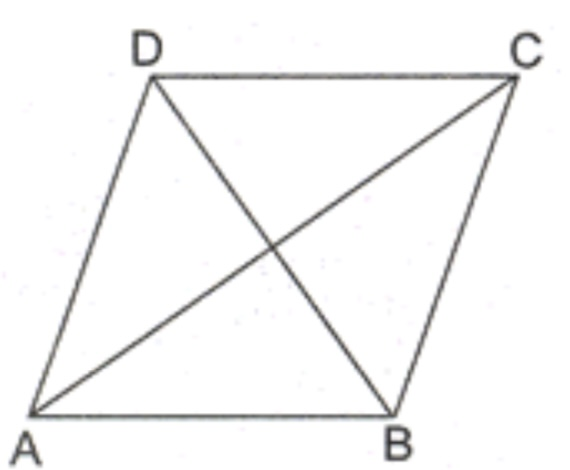
\includegraphics[width=70mm]{./images/IMG03.PNG}
          \caption{4}                                                                                                                                             \label{fig:}

 \end{figure}\\
Makeing  ue  of the above, prove the following:\\
in fig:4, $ABCD$ is a fig:4 rhombus. prove that $4AB^2 =  AC^2 +BD^2$.


\item Prove that I a line touch a circle and from the point of contact a chord is drawn, the angles
which this chord makes with the given line are equal respectively to the angles formed in the
corresponding alternate segments.
Using the above, do the following: \\
$AB$ is a diameter and $AC$ is a chord of a circle such that $\angle BAC=30^\circ$. The tangent at C
intersects $AR$ produced in a point I Prove that $BC = RD.$

\item A man standing on the deck of a ship, which is 10 m above the water level, observes the
angle of elevation of the top of a hill as 60° and the angle of depression of the base of the hill as
300. Calculate the distance of the hill from the ship and the height of the hill.

\item From a window $x$ meters high above the ground in a street, the angles of elevation and depression of the top and foot of the other house on the opposite side of the street are $\alpha$ and $\beta$ respectively. Show that the height of the opposite house is $x(1 + \tan \alpha \cot \beta)$ meters.






\end{enumerate}
\end{document}
